%&tex

\chapter{Real world}\label{chp:realworld}

In this chapter we finally apply our model to a real-world implementation of mobile robot lane
following. We give reasons as to why we chose the models and pre-processing used in our real-world
experiment. Next, we describe how each model performed in each track. A video of the robots on each
track is available online\footnote{\url{https://youtu.be}}.

\section{Control and inference}

Our main goal in this project was to be able to provide a fast, accurate and robust model for
self-driving that was capable of real-time measurement of uncertainty. Emphasis must be placed on
real-time, as a self-driving car ought to react at least as fast as a human. For this reason, we
chose to use a very simple control system that relied on fast and accurate inference to perform
well.

In~\cite{self-driving}, the robot's control system employed a command queue, in which the robot ran
an infinite loop where it only moved a fixed distance and then waited for inference to finish to
repeat itself. This method of self-driving evaluation nicely quantifies accuracy, but fails to
account for inference speed. Indeed, Moraes and Salvatore achieved $\approx$80\% accuracy with
deep-forward neural networks and $\approx$85\% with convolutional neural networks, but inference
took about 1.35 seconds, with binarized results taking faster average speeds of 0.6 seconds. In the
real-world, a self-driving car cannot afford to run a few meters, stop for inference, and then
continue for a few more. We account for this in our implementation.

A reactive control system was built whose input was based solely on commands given by an inference
model. Not only that, the speed of which these commands were given impacted heavily on its
performance. As mentioned in~\autoref{chp-harware}, the Brick receives a command and applies power
to its motors accordingly. Until another command is given by the Berry, the Brick repeats the same
command previously given. For instance, if the Brick was given a command to go straight, it will
continue to do so until a different order is otherwise given. This sort of control is able to
quantify how reliable is inference based not only on accuracy, but also speed of inference.

In~\autoref{chp:benchmarks}, we showed inference speed results based on a desktop computer with a
powerful CPU. When running the same models on the Berry, we found that although the binarized GD
architecture achieved 85\% accuracy and took about 0.3 seconds on a desktop PC, this speed went up
to 3.5 seconds on the Berry. This high increase is not only due to the power difference between the
two CPUs, but also by the need of real-time image pre-processing (in this case binarization)
directly from a live video.

This speed discrepancy forced us to discard several models due to slow inference. In fact, we found
that a model that took more than 0.15 seconds would take more than 1 second on the Berry.
Additionally, histogram equalization proved to severely decrease speeds, causing us to discard any
of its use in our real-world experimentations. We ultimately decided to use

\begin{enumerate}
  \item\label{item:setup-1} $Q_4$ and GD+d;
  \item\label{item:setup-2} $Q_6$ and GD+d;
  \item\label{item:setup-3} no pre-processing and GD+d.
\end{enumerate}

Inference times were about 0.7, 0.150 and 0.075 seconds for~\autoref{item:setup-1},
\autoref{item:setup-2} and \autoref{item:setup-3} respectively. Our experiments show that a high
accuracy but slow inference speed performs poorly on our setup. A low accuracy but fast prediction
speed model can behave erratically, but is able to correct itself because of its speed. We found
that a good balance between accuracy and speed performed the best. We will refer as Model 1, Model
2 and Model 3 the model and pre-processing done in~\autoref{item:setup-1}, \autoref{item:setup-2}
and \autoref{item:setup-3} respectively.

\section{Tracks}

We built three different tracks in order to evaluate how models behaved in different environments.
We assembled tracks in the same way as done in~\cite{self-driving}. In each track, A4 paper sheets
were placed in order to form road markings on both sides of the ``road''. In this section, we
describe each track and discuss how each model performed.

\subsection{Track 0}

The first track is a standard square shaped track. It is the simplest track we built in order to
evaluate turns and lines. The robot's objective is to complete a lap without going out of bounds.

All models were able to drive through the whole lap. We noticed that Model 1 was much slower in
terms of updating its state when compared to the other models. It particularly had trouble with
straight lines, as the model's slow inference speed prevented it from making small corrections and
thus propagated a sort of accumulated error at each attempted correction. Model 3 seemed to avoid
moving in a straight line, opting to zig-zag instead. This model's behavior was a constant in every
track. Model 2 was able to correctly turn and run lines with no apparent issue.

\begin{figure}[h]
  \centering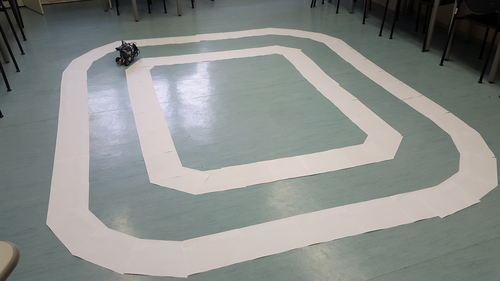
\includegraphics[width=0.9\textwidth]{imgs/track_0.png}
  \caption{Track 0 is a simple square shaped circuit.}
\end{figure}

\subsection{Track 1}

In this $\infty$-shaped track, the robot is supposed to travel through both conjoined circles,
alternating between the two of them without going out of bounds.

\begin{figure}[h]
  \centering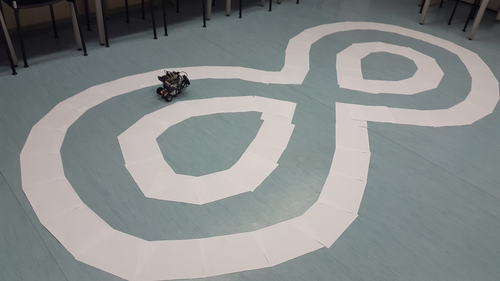
\includegraphics[width=0.9\textwidth]{imgs/track_1.png}
  \caption{Track 1 is an infinity shaped circuit.}
\end{figure}

Model 1 was unable to complete the lap, as once on the intersection of two circles, the robot kept
its course, repeating the same circle instead of the other. Model 2 completed the track perfectly.
Model 3 zig-zagged throughout the whole course, but was able to complete the track as well.

\subsection{Track 2}

The hardest of the tracks, it features sharp turns and irregular paths. One may map this artificial
scenario to the real-world challenge of roads in steep terrains, such as going down a mountain. An
additional challenge in this circuit is the proximity and otherwise intersection between road
markings that do not belong to the track the robot is currently on. This confuses the robot, as
depending on its position relative to the marks, it may incorrectly predict its next action.
Indeed, all models failed in this track directly of indirectly due to this.

\begin{figure}[h]
  \centering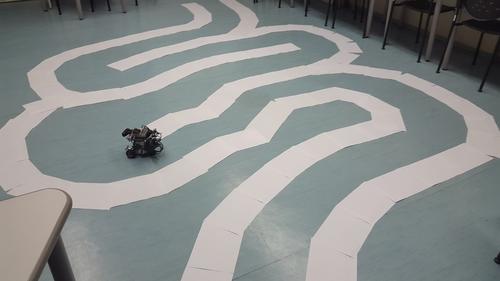
\includegraphics[width=0.9\textwidth]{imgs/track_2.png}
  \caption{Track 2 simulates a road going down a mountain.}
\end{figure}

Turns are identified by their order of appearance when travelling the pathway. Turns are
increasingly tighter as the road progresses. \autoref{fig:track-2-marks} marks these four turns
with visual aids colored in blue. We do the same for the three ambiguous road markings, coloring
them with red.

\begin{figure}[h]
  \centering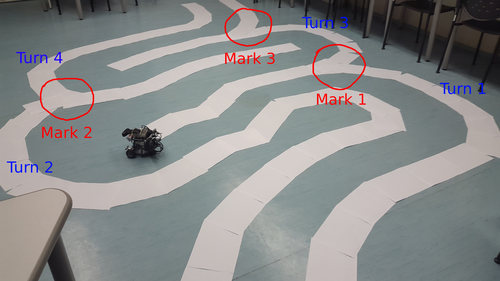
\includegraphics[width=0.9\textwidth]{imgs/track_2_marks.png}
  \caption{Track 2 ambiguous markings and sharp turns.}
\end{figure}

Model 1 failed due to both ambiguous road markings (particularly on Mark 1) and the first sharp
turn (Turn 1). Because it had slow inference, it was unable to correct itself. Model 2 managed to
go all the way down to Turn 3, however it got confused on Mark 3, mistaking it for a right turn.
Model 3 failed on Mark 2 due to the same reasons.

Track 2 was designed with the flaws of our system in mind. We knew beforehand our approach with
image classification does not take into account previous classifications. This causes ambiguous
markings to be misclassified when they could have been inferred from previous predictions.
Likewise, sharp turns prove to be a challenge for a robot that is only allowed to go forward, as
one misclassification may prove fatal. Nevertheless, Model 2 exceeded our expectations, managing to
correctly travel through Turn 1 and Turn 2, and correctly evading Mark 1 and Mark 2.
